\section{Architecture}

The architecture of our tools is illustrated in Figure ~\ref{fig:architecture}. Our tools are web-based and use standard web technologies such as HTML5, CSS3 and JavaScript. There is a main application that runs on the developer's desktop PC and provides the UI for our tools. Furthermore, a Chrome extension runs in the browser of the developer's machine that is responsible for coordinating parts of the integration with the  browser's debugging tools. This application is provided by a server that also coordinates the communication between devices and runs a small side application for the real devices. The server runs locally on the developer's machine. Furthermore, a local DNS server runs on the developer's machine that is responsible for creating different subdomains for the emulated devices. The application that is being tested is provided by an application server. The specifics of this server are up to the developer of the application. The only requirement is that the developer injects a small script that is hosted on our server at the top of each HTML page of the application.

\begin{figure}[H]
  \centering
    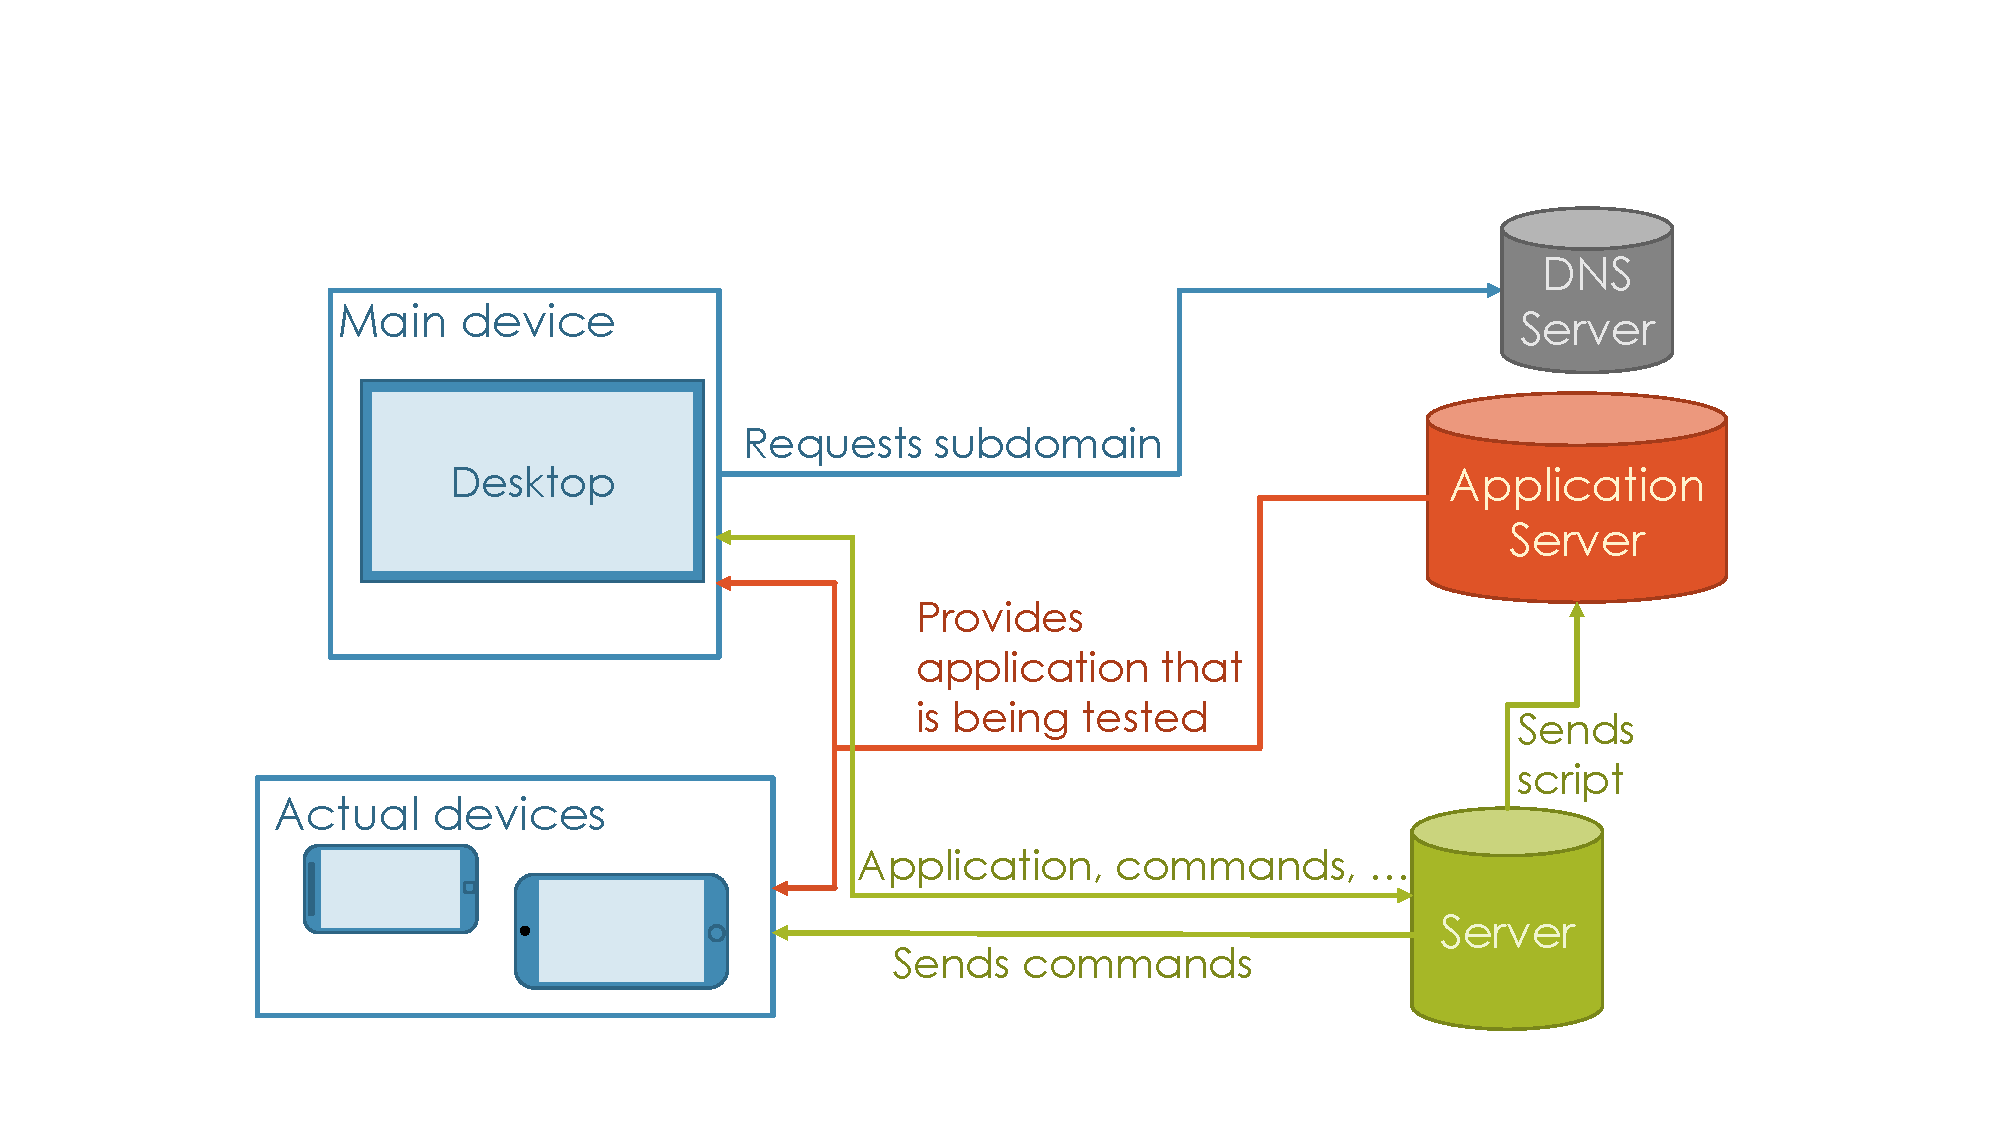
\includegraphics[width=1.0\textwidth]{images/architecture.pdf}
	\caption{Architecture of our tools}
	\label{fig:architecture}
\end{figure}

\section{Choice of Technologies}

Since our set of tools includes desktop devices as well as mobile devices, it should be platform-independent. Thus, our tools are implemented using standard web technologies, i.e. HTML5, CSS3 and JavaScript. This allows our tools to be run in any modern web browser without requiring installation of any additional software. The fact that cross-device applications are also typically web-based makes web technologies even more suited for our tools. Our tools do not rely on any database, instead local storage is used for the data that we want to store. Our set of tools only need to store three things:
\begin{itemize}
	\item Custom devices for emulation that were added by the developer.
	\item Device configurations.
	\item Event sequences for replaying.
\end{itemize}
All those things only need to be accessed by the developer that created them. Thus, it makes sense to only store the data locally. Furthermore, the amount of data that needs to be stored is rather low and does not require much storage. 

\subsection{Server Side}

On the server side, our tools use Node.js\footnote{\url{https://nodejs.org/en/}}. Node.js scales well with a large number of connections and has the advantage that both the client and server side are implemented using JavaScript. Thus, no data conversions are required. In our application, fast communication between the desktop PC and the connected real devices is required and Node.js fulfills those requirements. In order to facilitate our server and increase maintainability, we use Express\footnote{\url{http://expressjs.com/}}. 

For generating device IDs, we use shortid\footnote{\url{https://github.com/dylang/shortid}}. shortid generates short URL-friendly unique IDs. As each emulated device in our system gets a subdomain based on its ID, shortid is ideal for our purpose.

For communication between the server and client we rely on WebSockets, using the JavaScript library Socket.io\footnote{\url{http://socket.io/}}. Socket.io is better suited for our application than AJAX for multiple reasons: First, we need to be able to send push data to clients from the server for sending commands to devices and AJAX is intended to allow clients to pull data from the server. Also, data transfer with AJAX comes with a significant overhead because HTTP headers are transmitted with each piece of data. As we mentioned before, fast communication between the server and the devices is a requirement for our system and AJAX would not fulfill this requirement sufficiently. However, AJAX is used for communicating with the DNS server.

\subsection{DNS Server}

Our system requires a DNS server for registering the subdomains for the emulated devices. It should be easy to dynamically add new subdomains to the DNS server. Furthermore, the DNS server should forward any unknown domains to the standard DNS server. rainbow-dns\footnote{\url{https://github.com/asbjornenge/rainbow-dns}} fulfills both those requirements. It is a Node.js-based DNS server with an HTTP API that makes it trivial to register new domains from our application. When starting the server, the IP address of the standard DNS server can be set, allowing rainbow-dns to forward unknown domains to the standard DNS server.

\subsection{Client Side}

Bootstrap, jQuery, jQuery UI, jQuery.qrcode

\section{General Features}

In Figure ~\ref{fig:complete}, the complete interface of our set of tools can be seen.

\begin{figure}[H]
  \centering
    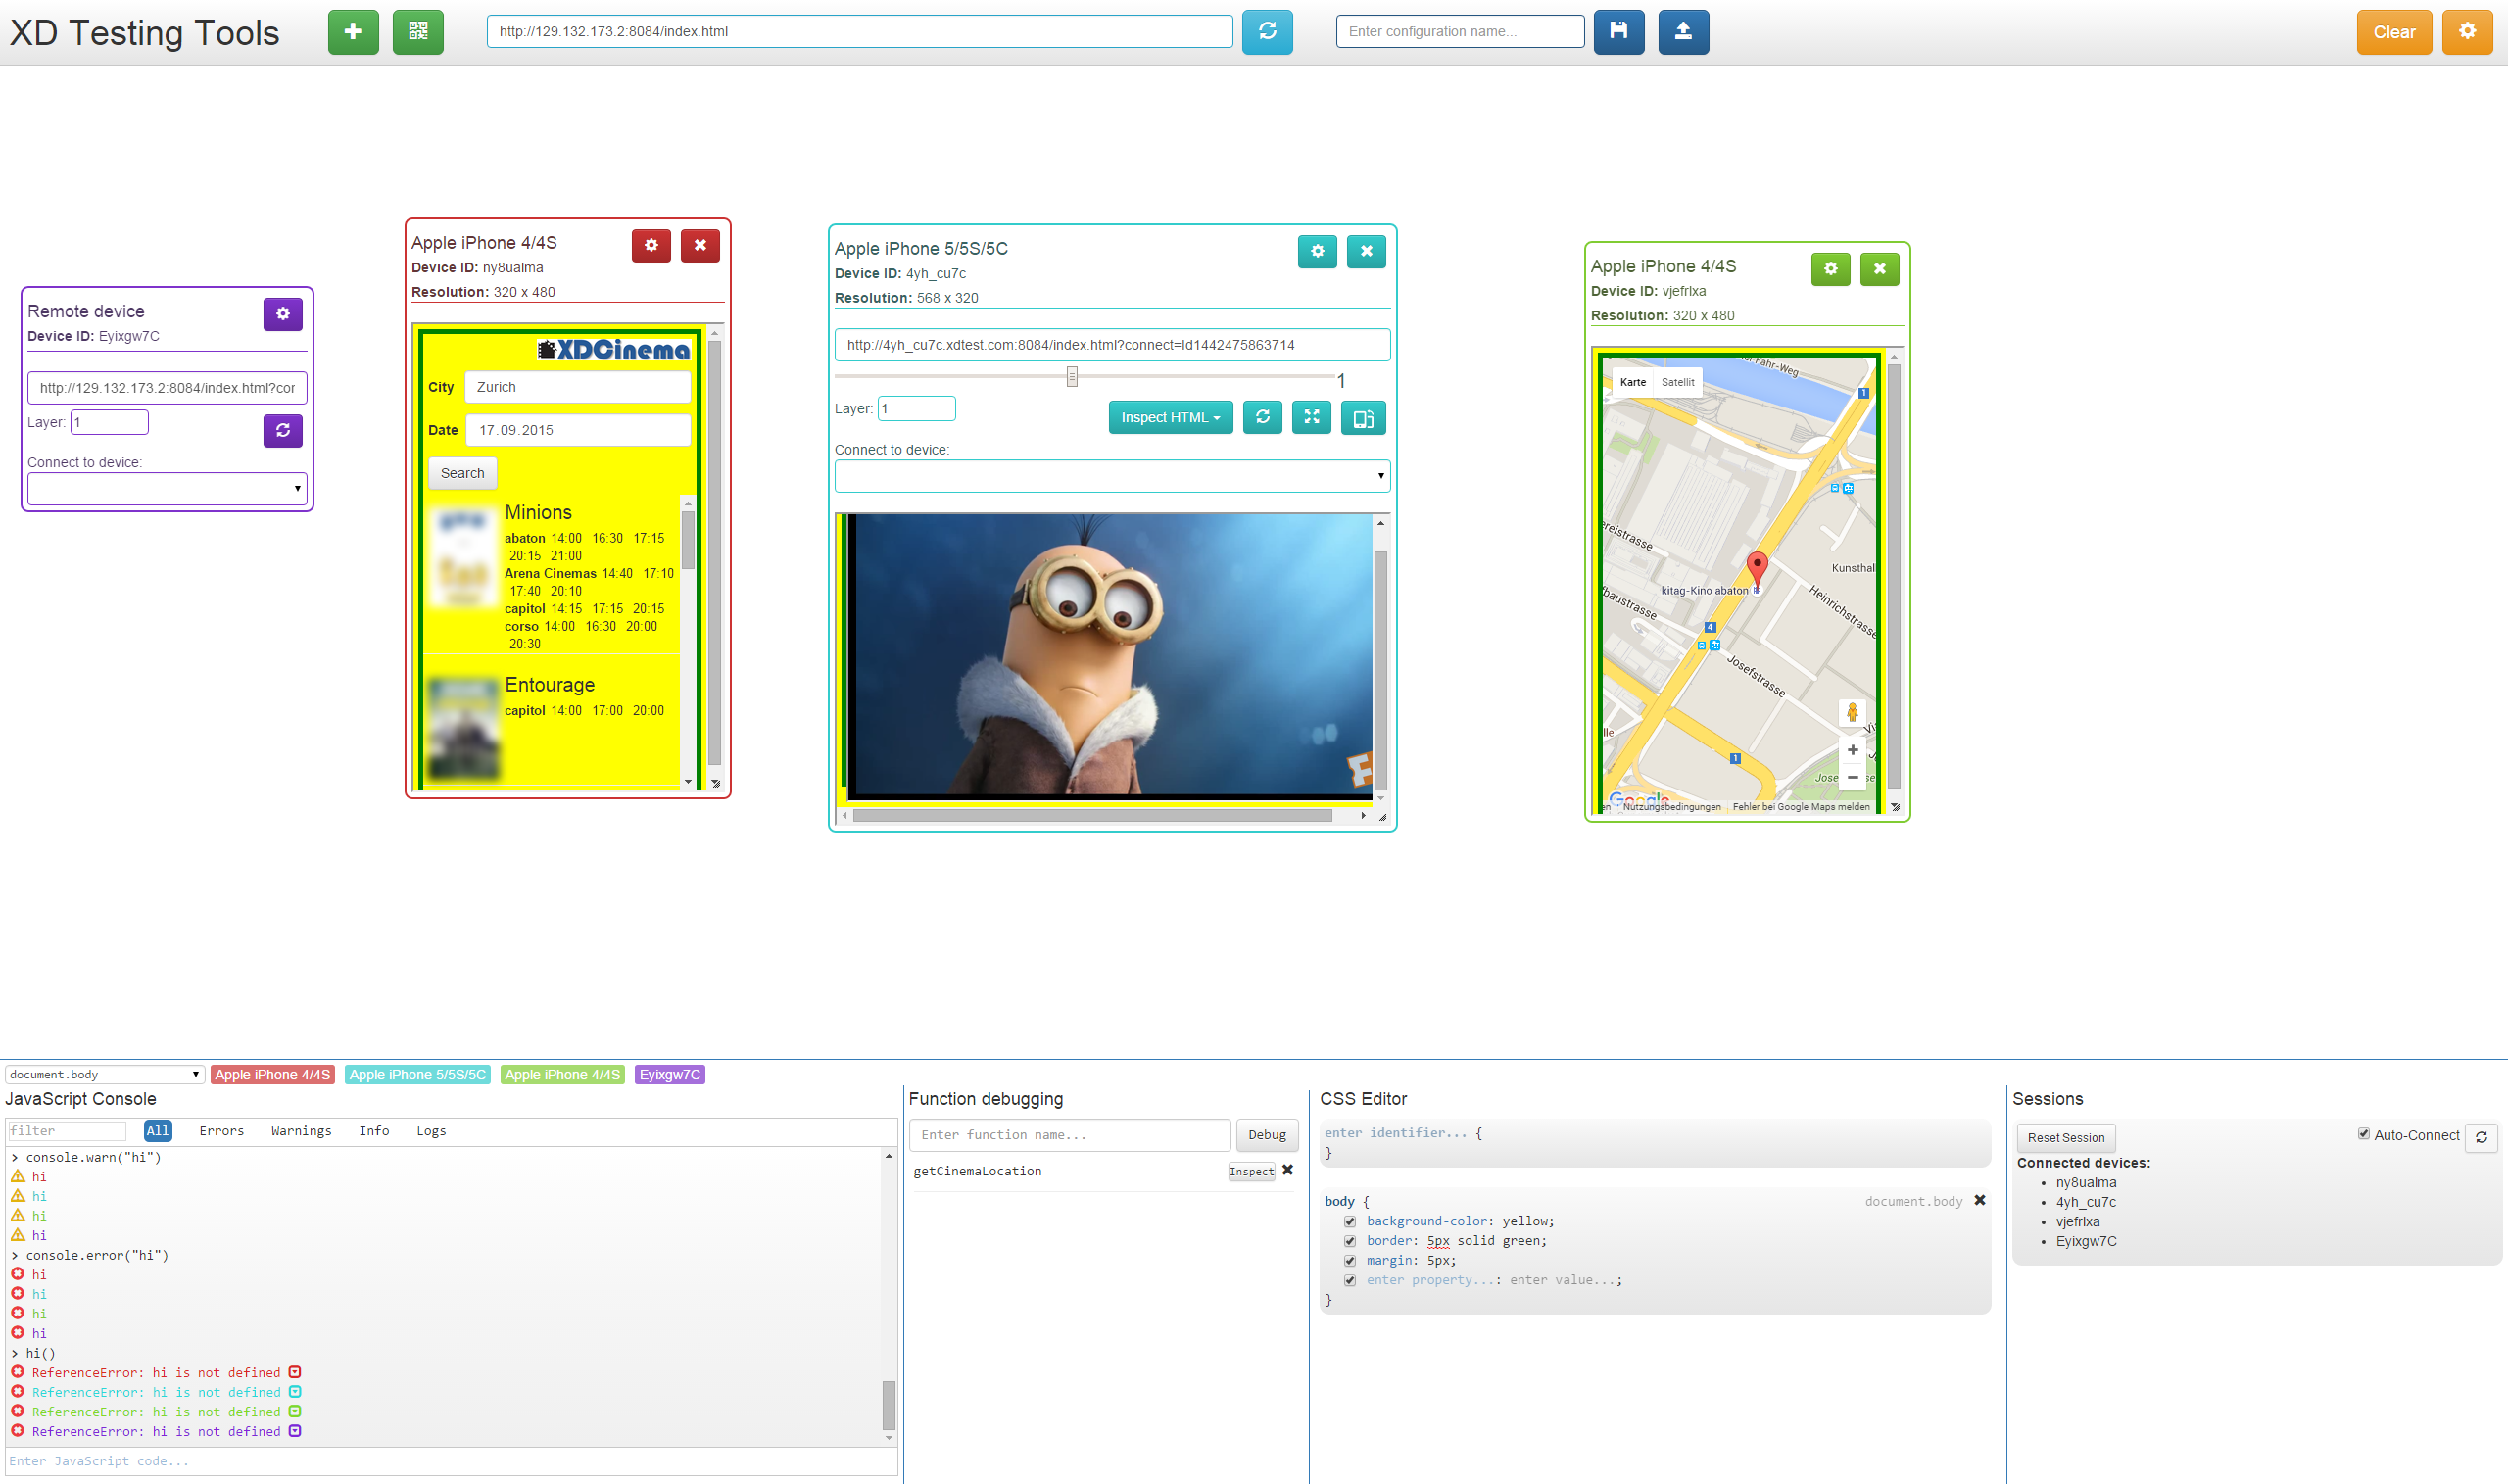
\includegraphics[width=1.0\textwidth]{images/screenshots/complete.png}
	\caption{The complete interface}
	\label{fig:complete}
\end{figure}

Figure ~\ref{fig:complete_remote} shows a screenshot of the remote device that is connected to our system in the screenshot shown before.

\begin{figure}[H]
  \centering
    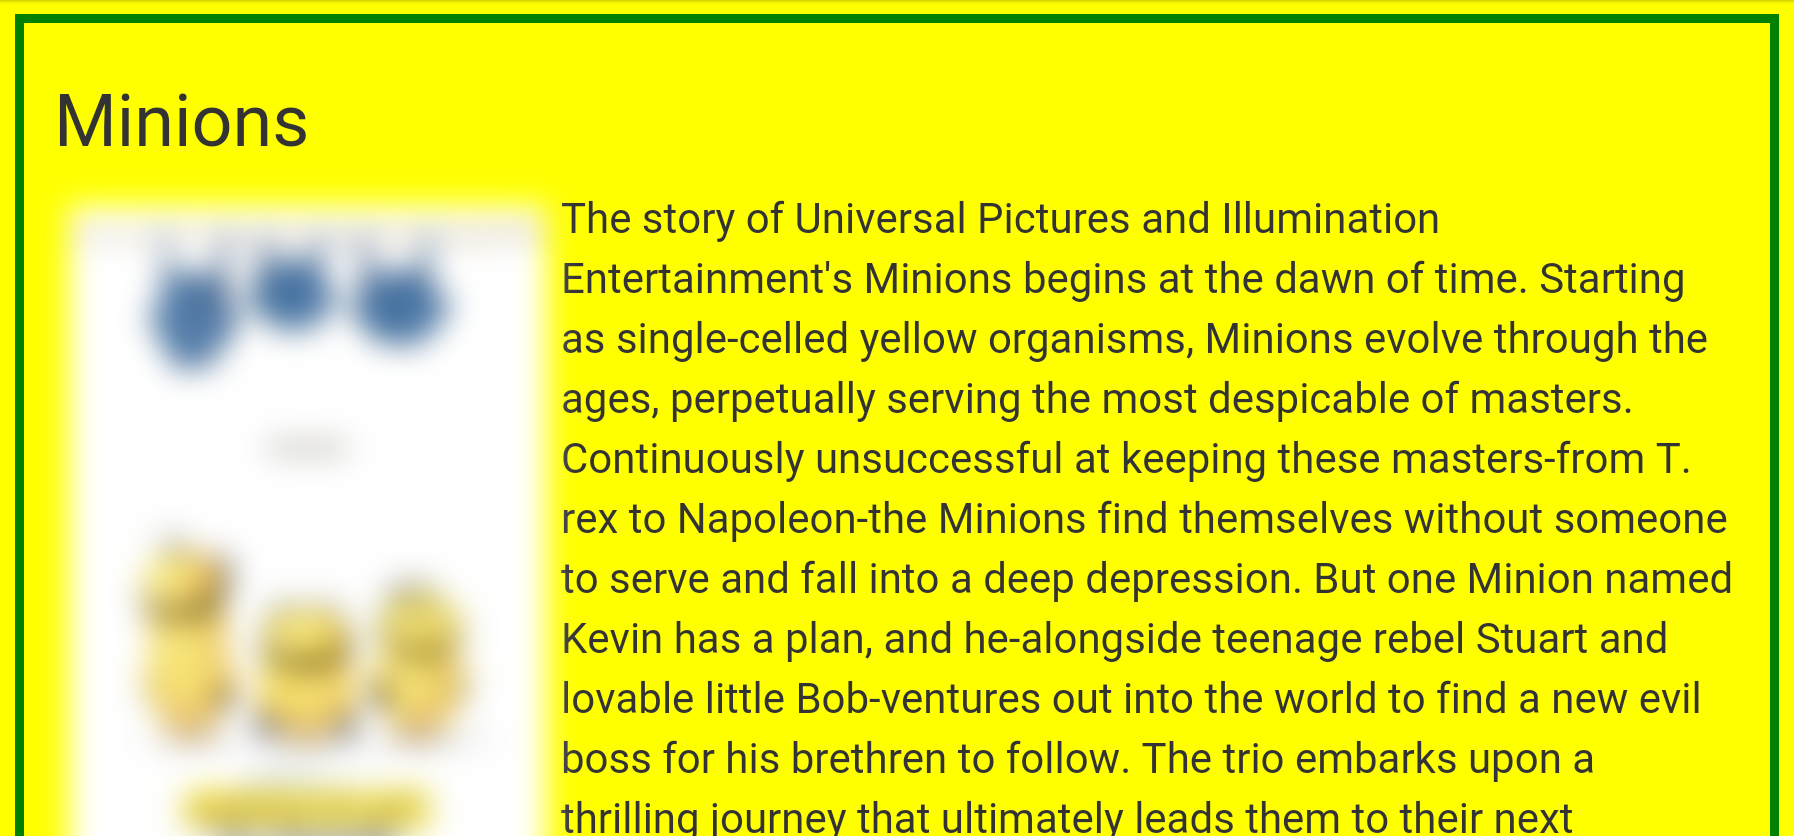
\includegraphics[width=0.8\textwidth]{images/screenshots/complete_remote_2.png}
	\caption{The connected remote device}
	\label{fig:complete_remote}
\end{figure}

\section{Device Emulation}

Device emulation is emulated using iframes: Each emulated device has its own iframe that loads the application that is being tested. However, loading the same domain inside multiple iframes would lead to the sharing of session and persistent data between all emulated devices. We have already described how developers tackle this problem and the limitations of those solutions. For our tools, we created a more scalable and robust solution. When an emulated device is created, it is assigned a unique ID. Based on this ID, a unique subdomain is registered with the local DNS server. All those subdomains will still point to the same application, but as the application is accessed through different domains, no data is shared between the emulated devices. Domains that are unknown to the local DNS server are forwarded to the standard DNS server. Each iframe has the resolution of the device that it emulates. Currently, only the resolution of the target devices is emulated, but in the future, our tools could be extended to support emulation of more aspects. In Figure ~\ref{fig:emulated_device}, an emulated device can be seen.

\begin{figure}[H]
  \centering
    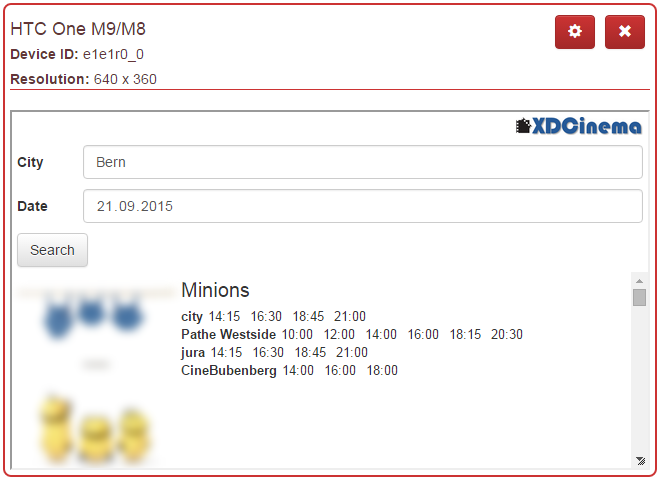
\includegraphics[width=0.8\textwidth]{images/screenshots/emulated_device_3.png}
	\caption{An emulated device}
	\label{fig:emulated_device}
\end{figure}

Apart from its unique ID, each device also has a unique color. The border of an emulated device is colored with this color and the color is used in multiple other places for identifying the device. The devices also have a settings menu. In the settings menu, the developer can configure the following things:
\begin{itemize}
	\item The URL of the device.
	\item The scaling of the device.
	\item The orientation of the device.
	\item The layer of the device, i.e. the z-index. 
	\item The iframe of the device can be refreshed.
	\item The developer can inspect the HTML of the device.
	\item The developer can connect the device to another device by choosing it in a dropdown menu.
\end{itemize}
The device's settings are not constantly used by the developer and showing them at all times would occupy valuable screen space. Thus, the setting menu can be extended and collapsed by the developer by clicking a button. The scaling of the device is set using the CSS property "transform", e.g. by setting "transform: scale(0.5)" to scale a device to half its usual size. Using the "transform" property does not change the resolution of the iframe of the emulated device, only the space that the iframe takes up. Thus, the layout of the emulated device remains intact even if it is scaled down. If the developer instead wants to change the resolution of a device, they can click in the bottom-right corner of the iframe and drag to increase or decrease the resolution. This is realized using jQuery UI's Resizable\footnote{\url{https://jqueryui.com/resizable/}}. An example of a settings menu can be seen in Figure ~\ref{fig:settings_menu}. 

\begin{figure}[H]
  \centering
    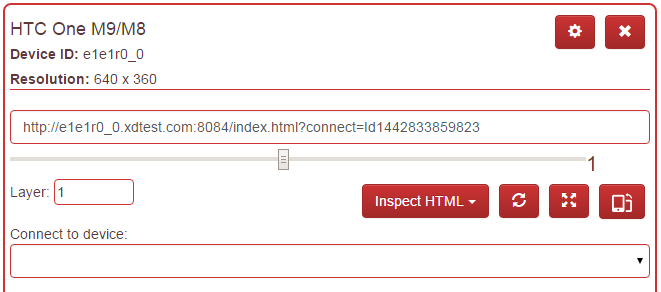
\includegraphics[width=0.8\textwidth]{images/screenshots/settings_menu_2.png}
	\caption{Settings menu of an emulated device}
	\label{fig:settings_menu}
\end{figure}

The devices can be moved by the developer as desired. Using HTML5's Drag and Drop\footnote{\url{http://www.w3schools.com/html/html5_draganddrop.asp}}, our tools allows the developer to click on the header of the device and then drag it to the desired location. 

\section{Connecting Real Devices}

Real devices can be connected by scanning a QR code or opening the URL. Once a real device has loaded the URL, the application that is being tested is shown in a full-screen iframe on the device. The developer can use the application on the real device, but everything relating to our tools is coordinated through the main application. Each connected real device is represented by a proxy within our main application. The proxy of the real device also contains a settings menu, but no iframe is shown in the main application for the real device. The settings menu is also missing a few things:
\begin{itemize}
	\item Scaling of the device: There is no need to scale real devices, as no iframe is shown in the main application.
	\item Switching orientation: The orientation of a real device can be switched on the real device itself by simply rotating the real device.
	\item Inspecting the HTML: The main application has no access to the HTML of the real device, thus it cannot be inspected.
\end{itemize}
Figure ~\ref{fig:settings_menu_remote} shows the settings menu of a remote device. The settings menu only contains interface elements for setting the URL of the device, the refresh button, the layer input field and the dropdown menu for connecting the device to other devices. If the developer issues any command on the main device, e.g. refreshing the iframe of the real device, the command is first sent to the server and then forwarded to the target device. 

\begin{figure}[H]
  \centering
    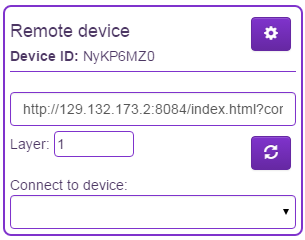
\includegraphics[width=0.5\textwidth]{images/screenshots/remote_device.png}
	\caption{Settings menu of a remote device}
	\label{fig:settings_menu_remote}
\end{figure}

The proxy of the real device can be moved around just like the emulated devices and its settings menu can  also be collapsed and extended.

\section{Shared JavaScript Console}

The shared JavaScript console aggregates the console outputs of all devices and allows the developer to send commands to all devices. The following types of logging messages are forwarded:
\begin{itemize}
	\item console.log
	\item console.debug
	\item console.warn
	\item console.info
	\item console.error
	\item console.count
	\item console.dir
	\item console.assert
\end{itemize}
In the script that is injected in the application being tested, those functions are overwritten by a new function. The new function first sends the content and type of the logging message to our server and then calls the original logging function. For forwarding JavaScript errors, an event handler is assigned using "window.onerror" that is called whenever a JavaScript error occurs. The error is then forwarded to our server, together with the stack trace if available. 

Depending on the type of message that is sent (error, warning, info, log and all others), a different symbol is used in front of the message being displayed in the console. The message itself is colored in the color of the device that sent it. If a device is deactivated, it does not forward any messages or errors anymore and all existing messages are filtered out. The console can be filtered by the four types of messages mentioned above. All messages that do not have the symbol that represents this type of message are hidden as long as the filtering is active. If the developer types a string to filter by, all messages are checked and if a message does not contain this string anywhere, it is hidden.

If the user types a command into the console, the command is sent to all active devices. Inside the script in the application, the JavaScript function "eval" is called with the command string as argument. The return value of the command is sent back to the server and displayed in the shared JavaScript console.

The screenshot in Figure ~\ref{fig:js_console} shows the shared JavaScript console including a few examples of how to use it. First, the developer tries to call a function on all devices but makes a typo. Because the function with the typo in the name does not exist, an error message is displayed by all devices. The developer then notices the typo, types the correct function and sees the return value of the functions (the coordinates of a cinema). Finally, the developer wants to see which roles have been assigned to the devices. They type the name of the variable that contains the roles and the value of this variable on all devices is shown in the console.

\begin{figure}[H]
  \centering
    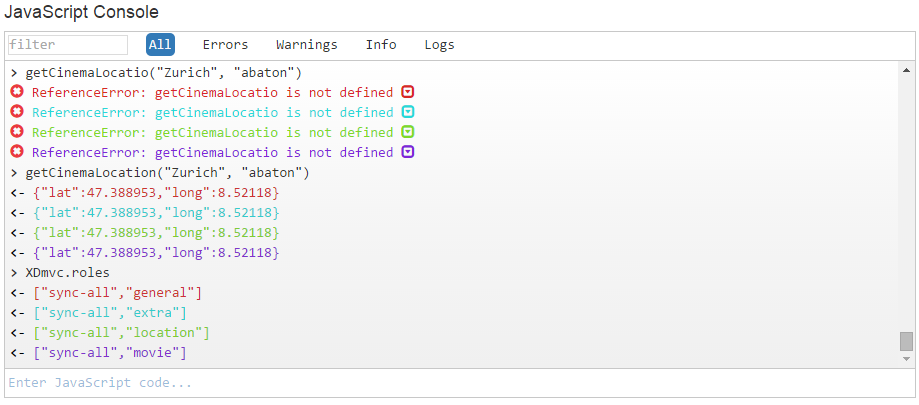
\includegraphics[width=1.0\textwidth]{images/screenshots/js_console_2.png}
	\caption{Shared JavaScript console}
	\label{fig:js_console}
\end{figure}

\section{Function Debugging}

For function debugging, the Chrome extension is required. The developer has access to an input field where they can type the name of the function they want to debug. When the developer adds a function to debug, a command is sent to each activated emulated device. As soon as a device receives the name of a function to debug, it overwrites the function by another function and stores the original function. The function that overwrites the original function first highlights the device with a semi-transparent green overlay, then calls the original function and stores the return value, then it removes the highlighting from the device and returns the return value. After the function is overwritten, it sends a message back to the server that it is ready for debugging. The server then sends a command to the Chrome extension with the name of the original function. The Chrome extension receives the command and the URL of the device the message originated from. The Chrome extension then adds the function for debugging using the function name and the URL of the frame that represents the device as parameters. 

When the debugged function is now called on one of the devices that the developer wants to debug, the overwriting function is called first and highlights the device. Then, the original function is called and interrupted right at the beginning so the developer can debug the function. After finishing debugging, the function call returns and the device can be unhighlighted. Figure ~\ref{fig:function_debugging_complete} shows a screenshot while a function is debugged. In the screenshot, the highlighted device, the DevTools with the debugged function opened and the list of debugged functions can be seen.

\begin{figure}[H]
  \centering
    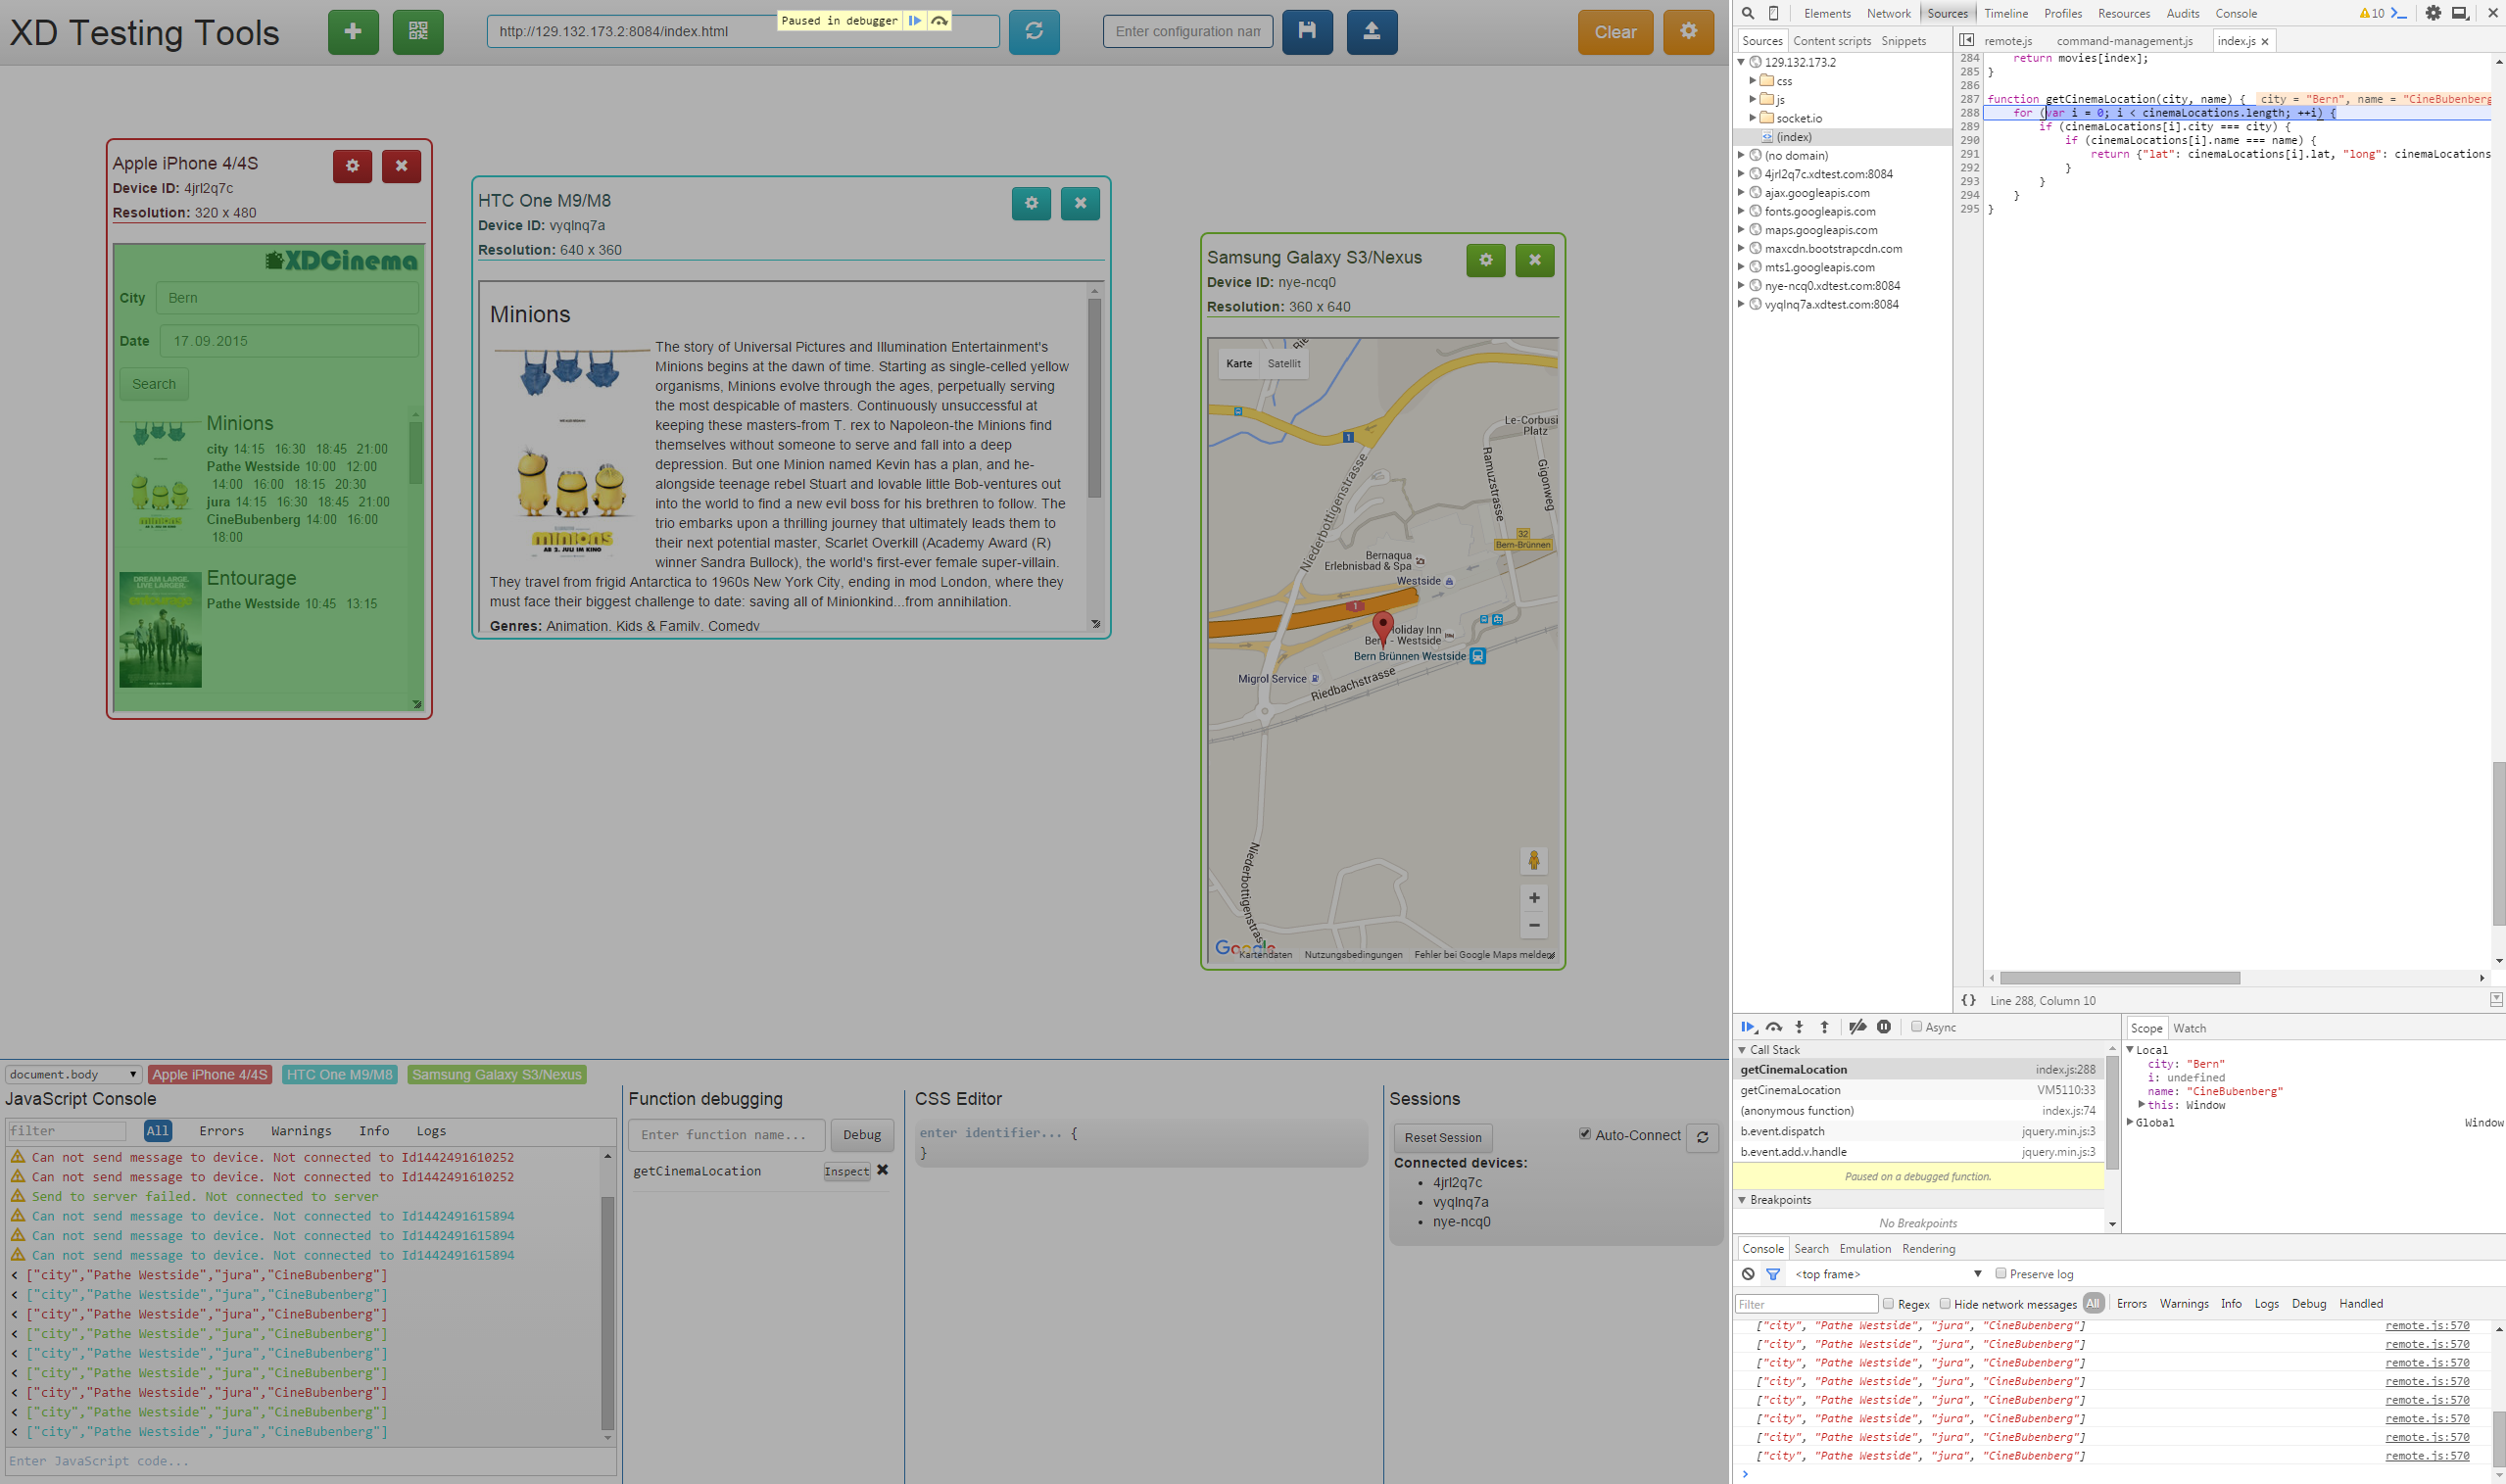
\includegraphics[width=1.0\textwidth]{images/screenshots/function_debugging_complete.png}
	\caption{The complete interface while debugging a function}
	\label{fig:function_debugging_complete}
\end{figure}

If the developer is done debugging a function, they can remove it from the list of debugged functions and the original function is restored inside the script. Additionally, the developer can also just inspect the function without it being called by clicking on a button in the list of debugged functions. Then, the function is opened on a random device. 

Apart from function debugging, the Chrome extension is also used for inspecting the HTML of the device. The developer can click on a button in the settings menu of an emulated device to jump directly to the body of the HTML of the device inside the Chrome DevTools. When the developer clicks on the button, a command is sent to the server and then forwarded to the DevTools. The DevTools call the function "inspect" that is part of the DevTools API with the URL of the frame of the device and "document.body" as arguments.

\section{Shared CSS Editor}

For the CSS editor, a stylesheet is created and added to the document inside the script. If the developer adds a new rule to the CSS editor, a command is sent to all devices and the rule is added to the stylesheet. The rules are also stored in an array of CSS rules and the stylesheet is rewritten every time something changes for simplicity. The developer can enable and disable rules. If a rule is disabled, it is removed from the stylesheet; if it is enabled again, it is re-added to the stylesheet.

Figure ~\ref{fig:css_editor} shows a screenshot of the CSS editor in action. In this screenshot, some CSS rules are added to the body element of all devices.

\begin{figure}[H]
  \centering
    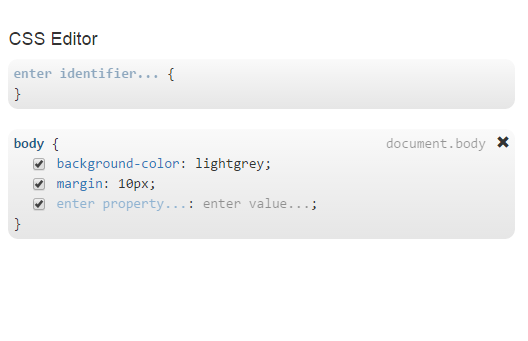
\includegraphics[width=1.0\textwidth]{images/screenshots/css_editor.png}
	\caption{Shared CSS Editor}
	\label{fig:css_editor}
\end{figure}

In Figure ~\ref{fig:css_applied}, the effects of the CSS shown in the screenshot above are shown. 

\begin{figure}[H]
  \centering
    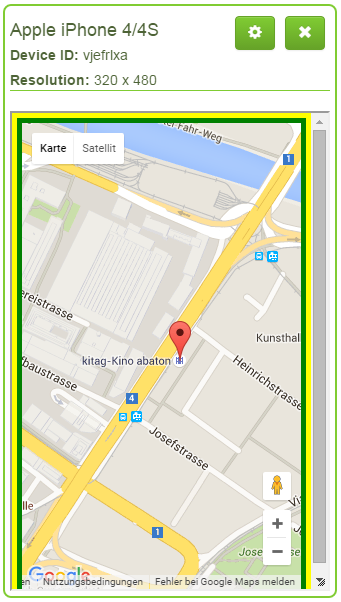
\includegraphics[width=0.5\textwidth]{images/screenshots/emulated_device_2.png}
	\caption{CSS applied to emulated device}
	\label{fig:css_applied}
\end{figure}

\section{Record/Replay}

As soon as the script is loaded, event handlers are assigned for all relevant events that we want to record. However, the event handlers do not do anything as long as recording has not started yet. When the developer starts recording, all events are logged to an array. After finishing recording, the array of events is sent to the server and then to the main application. The event handlers are already assigned when loading the script because otherwise other scripts would get a chance to assign event handlers and thus receive events before our script. Furthermore, the event handlers are assigned to the document itself and capturing, thus no other element can receive an event first. This is important because otherwise the page could be modified before we receive the event or the event could even be stopped from propagating. Before sending event sequences back to the server, all circular structures are removed. All other event properties are kept so the events can be replayed accurately.

The event sequences should be replayable on other devices than the recording devices, therefore some way of determining the target of the event is required. Whenever an event handler is triggered, the DOM hierarchy is traveled up from the target of the event until an ID is reached. From this ID, we can reach the target element by taking the correct child until the target element is reached. From this, we can derive a hierarchy that describes how to reach the target element on a device and replaying the event on another device becomes possible.

After the main application receives an event sequence, the sequence is visualized. Drag and drop can be used to adjust the timing of the event sequences on the devices. Event sequences can also be moved to other devices using drag and drop. Event sequences can be saved to local storage for later use. Because all events require some space when visualized, events that happen close together in time are grouped together. Event sequences can also be split by clicking between two groupings of events.

Furthermore, the developer can add breakpoints to the replaying timing. By clicking at a certain point in time, a breakpoint is set at that time. When the developer starts replaying, the event sequences assigned to a device are sent to the device along with the list of breakpoints. The events that happen before the first breakpoint are then triggered using "setTimeout". If a breakpoint is reached, a message is sent to the main application and the breakpoint that was reached is highlighted. After the developer chooses to continue, a message is sent to all replaying devices telling them to continue event replaying until the next breakpoint is reached. After the last breakpoint has been reached, the event replaying continues until all events have been replayed. 

All events are replayed using the properties recorded in the event sequences. Using the hierarchy computed when recording, the target element of the event is determined. For most events, replaying with the properties logged when recording is enough for realistically reproducing the events. However, some events require a bit more work. Replaying key events is possible, but no text is written into input fields. In addition to the key events, we also need to replay a text event using the correct char code. Scrolling events also do not scroll. Thus, we also log the scrolling position after a scrolling event occurs and manually set it after replaying the event. Furthermore, the backspace key cannot be reproduced with neither text events nor key events. Thus, we manually determine the position of the caret if the backspace key is pressed and delete the last character before the caret when replaying. 

Consider Shadow DOM for event hierarchy

\begin{figure}[H]
  \centering
    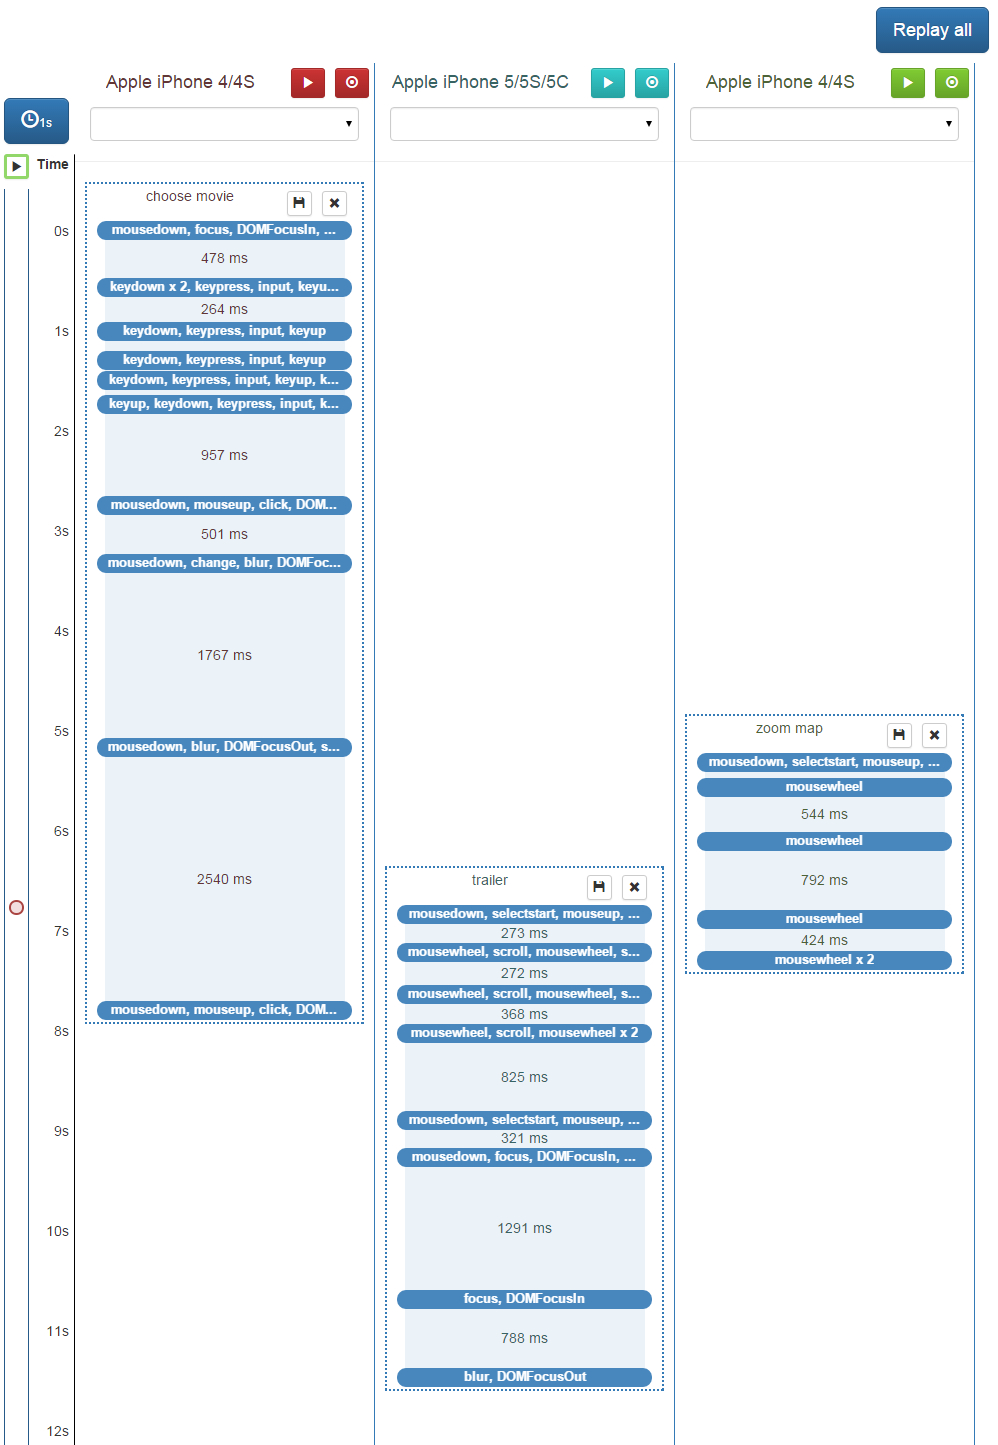
\includegraphics[width=1.0\textwidth]{images/screenshots/record_replay.png}
	\caption{Record and Replay}
	\label{fig:record_replay}
\end{figure}